% Waiting for Eloïse report template
% We need better display
% Sommaire inherited from projet_SGBD_rendu19.pdf

\documentclass[a4paper,10.5pt]{article}
\usepackage[utf8]{inputenc}
\usepackage[T1]{fontenc}
\usepackage[french]{babel}
\usepackage[top=2cm, bottom=2cm, left=2cm, right=2cm]{geometry}
\usepackage{hyperref}

%pictures
\usepackage{graphicx}

%maths
\usepackage{amsmath}
\usepackage{amssymb}
\usepackage{mathtools}
\usepackage{empheq}



\begin{document}
\noindent
\begin{minipage}{0.20\textwidth}

\includegraphics[width=\textwidth]{logo}
\end{minipage}
\hfill
\begin{minipage}{0.71\textwidth}
Système de gestion de Base de Donnée \hfill Nov. 2019\\

\begin{center}
{\Large \textbf{Projet}}

\vspace{0.5em}
 \large Melvin \bsc{Even} \quad Pierre \bsc{Pavia} \quad Maëlle \bsc{Toy-Riont-Le-Dosseur} \quad Lucas \bsc{Henry}
\end{center}\vspace{0.3em}


\end{minipage}\\

\noindent
\rule{\linewidth}{0.5mm}
\setcounter{section}{1}

\section{Modélisation des données}
\subsection{Description du contexte de l'application}

Les jeux de cartes à collectionner sont un élément important de la pop-culture de ces dernières années, et aussi un marché économique digne d'intéret. En effet, avec la popularisation de jeux comme Pokémon, Magic ou Yu-Gi-Oh depuis les années 90, ce sont de plus en plus de jeux et de joueurs qui se créent et qui se développent.

L'objectif est ici de créer une base de données correspondant à un de ces jeux de cartes à collectionner. Nous devons être capable d'y enregistrer quelles sont les versions différentes d'une même carte, et de calculer la valeur (ou la 'cote') d'une carte, à partir notamment de sa date de publication, du nombre d'exemplaires à laquelle elle a été tirée, et de son état.

Nous allons aussi répertorier chacun des matchs opposant les joueurs, avec l'endroit où ils ont lieu et le nom du vainqueur. Pour faire ça, nous devons donc enregistrer une liste des différents joueurs.

Les joueurs doivent aussi pouvoir les regrouper par mains (ou 'decks') pour pouvoir retrouver quelle carte était possédée par quel joueur, pour chacune des parties.

\subsection{Modèle entité-association}

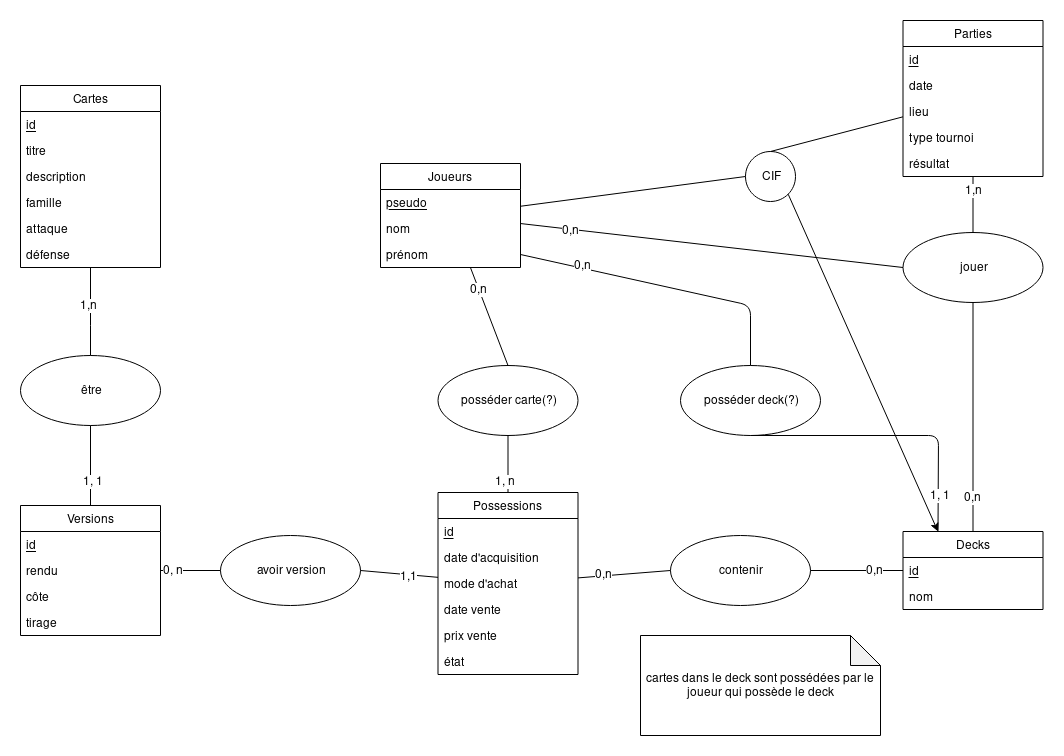
\includegraphics[width=\textwidth]{modele_conceptuel.png}

\subsection{Liste des opérations prévues sur la base}

Voici la liste des actions retenues sur la base de donnée~:

Consultation~:

\begin{itemize}
  \item Liste des cartes d’un certain type.
  \item Liste des cartes qui ne font partie d’aucun deck.
  \item La liste des joueurs qui n’ont fait aucune partie (ce sont juste des collectionneurs).
\end{itemize}

Statistiques~:

\begin{itemize}
  \item La liste des joueurs, avec le nombre de cartes qu’ils possèdent.
  \item La liste des joueurs classés par ordre décroissant selon la valeur de
    leur collection (la valeurd’une carte étant estimée au produit de sa côte
    par son état).
  \item La liste des cartes avec le nombre de joueurs qui les utilisent dans
    leurs decks.
  \item La liste des joueurs possédant le plus de cartes rares (date
    d’impression antérieure à 2000 ou tirage inférieur à 100).
  \item La liste des familles de carte, avec, pour chaque famille, la
    caractéristique dans laquelle cette famille a le meilleur niveau.
\end{itemize}

Mise à jour~:

Il faut implémenter l'ajout et la suppression pour les éléments suivants~:
\begin{itemize}
  \item La base de donnée.
  \item Un joueur.
  \item Un deck.
  \item Une carte.
  \item Une version de carte.
  \item Une possession d'une version de carte.
  \item Une partie.
\end{itemize}

\section{Schéma relationnel}
\subsection{Passage au relationnel}

La conversion des entités donne rapidement les premières règles suivantes :\\
\\
\texttt{Cartes(\underline{id\_carte}, titre, description, famille, attaque, defense)} \\
\texttt{Versions(\underline{id\_version}, \#id\_carte, rendu, cote, tirage)} \\
\texttt{Joueurs(\underline{pseudo}, nom\_joueur, prenom\_joueur)} \\
\texttt{Possessions(\underline{id\_possession}, \#pseudo, \#id\_version, date\_acquisition, mode\_achat,\\ date\_vente, prix\_vente, etat)} \\
\texttt{Decks(\underline{id\_deck}, nom\_deck, \#pseudo)} \\
\texttt{Parties(\underline{id\_partie}, date\_partie, lieu\_partie, type\_tournoi, resultat\_partie)} \\

Ensuite, en observant les cardinalités, on se rend compte qu'il est nécessaire de créer les deux relations supplémentaires suivantes. \\
\\
\texttt{Jeu(\underline{id\_partie}, \underline{id\_deck}, \underline{pseudo})} \\
\texttt{Appartenance(\underline{id\_possession}, \underline{id\_deck})} \\

\subsection{Contraintes d'intégrité, dépendances fonctionnelles}
Après l'ajout des contraintes : \\
\\
\texttt{Cartes(\underline{id\_carte} [U, NN], titre [NN], description [NN], famille [NN], attaque [NN], defense [NN])} \\
\texttt{Versions(\underline{id\_version} [U, NN], \#id\_carte [U, NN], rendu [NN], cote [NN], tirage [NN])} \\
\texttt{Joueurs(\underline{pseudo} [U, NN], nom\_joueur [NN], prenom\_joueur [NN])} \\
\texttt{Possessions(\underline{id\_possession} [U, NN], \#pseudo [U, NN], date\_acquisition [NN], mode\_achat [NN], date\_vente, prix\_vente, etat [NN])} \\
\texttt{Decks(\underline{id\_deck} [U, NN], nom\_deck [NN], \#pseudo [U, NN])} \\
\texttt{Appartenance(\underline{id\_possession} [U, NN], \underline{id\_deck} [U, NN])} \\
\texttt{Parties(\underline{id\_partie} [U, NN], date\_partie [NN], lieu\_partie [NN], type\_tournoi [NN], resultat\_partie [NN])} \\
\texttt{Jeu(\underline{id\_partie} [U, NN], \underline{id\_deck} [U, NN], \underline{pseudo} [U, NN])} \\

\textit{Contraintes : U = Unique, NN = Non nul}
% contrainte pour la table Appartenance : les entités représentées par les clés étrangères #id_possession #id_deck doivent contenir la même clé étrangère #pseudo

\subsection{Shéma relationnel en $3^e$ forme normale}

\section{Implantation}
\subsection{Création de la base de donnée}
\subsection{Implémentation des commandes SQL}

\section{Utilisation}
\subsection{Description de l'environnement d'exécution}
\subsection{Notice d'utilisation}
\subsection{Description des interfaces éventuelles}

\end{document}
